\chapter{Electronic Transitions of Europium}\label{ch:eu_theory}

Europium is a peculiar metal. Lanthanide metals have a complex
electronic structure consisting of an incomplete \textsl{4f} electron
shell, and many lanthanides, including europium, are highly reactive
\cite{Cooley:1946tv,Rard:1985tb}. These properties create a tricky
spectroscopic problem: europium has very low absorption cross sections in the
visible due to its electronic structure, and europium's reactivity means that
it is difficult to acquire lone europium to detect. This means that to analyse
europium in a solution it must be present at relatively high concentration in
a medium that europium does not react with.

\marginpar{Lower concentrations of europium can be measured in the UV.}

Using \ac{BBCEAS} it is possible to detect europium in a liquid sample at lower
concentrations than what is published in the literature.  The broad spectral
and simultaneous acquisition nature of \ac{BBCEAS} allows several spectral
features in the visible to be measured simultaneously.

While europium is challenging to characterise, it has a valuable
property: europium's photoluminescent quantum yield is nearly one
\cite{Scotognella:2009jo,Moudam:2009in, Bunzli:2005ic}, and the fluorescence
emission can be spectrally very narrow \cite{Werts:2002fs}. The quantum yield
is an important parameter in engineering uses for europium, yet this property
has not been explored well in the past due to the difficulty of extracting
information from fluorescence measurements \cite{Werts:2002fs}. By measuring
the absorption characteristics of europium using \ac{BBCEAS}, it is possible to
obtain a greater understanding of the fluorescence pathways and how to alter
them.

Europium also readily forms coordination complexes as both monodentate and
polydentate ligands
\cite{Kirby:1983cl,Sveshnikova:2000cr,Werts:2002fs,Bunzli:2005ic,Scotognella:2009jo,Moudam:2009in}. The fluorescence of europium, combined with a coordination complex, can be used
to create sensitive labels
\cite{Harma:2010dm,Pihlasalo:2010el,InstituteofBiomedicine:2011vt,Pihlasalo:2011ju,Pihlasalo:2012cq,Pihlasalo:2012en},
to create OLEDs with high spectral purity\cite{Moudam:2009in}, and as
luminescent solar concentrators\cite{Moudam:2009in,Wilson:2010hs}.

This chapter will explore the current understanding of europium's electronic
transitions and how to derive additional information such as quantum yields
and radiative lifetimes about europium complexes using \ac{BBCEAS}. At the
end of this chapter is a discussion about how it is possible to combine
\ac{BBCEAS} with europium complexes to create a highly sensitive protein
detection technique that can not only detect trace concentrations of proteins
but also indicate which proteins are in a solution.



\section{Theory of Lanthanide electronic transitions}\label{sec:theory_eu}

Lanthanide ions contain an open \textsl{4f} electronic orbital which leads to
many strange phenomena that are difficult to describe with standard quantum
mechanical models\cite{Wybourne:1968ez}. In the 1960s, researchers Judd and
Ofelt introduced simple assumptions to make the calculation of the electronic
wave functions simpler \cite{Judd:1962uq,Ofelt:1962kd}. Their simplifications
were successful in theoretically predicting the energy levels of different
electron configurations.

However, there exist electronic transitions that are still difficult to
understand because they are classically \emph{forbidden}. Some transitions are
forbidden due to a transition between two ground total angular momentum states
(noted as $ J=0 \leftrightarrow J'=0 $), while many others are forbidden due to
a change in the total spin $\Delta S \neq 0$. As such, these transitions must
occur due to higher order effects, such as electron configuration interaction
for the $^7F_0 \leftrightarrow ^5D_0$ transition \cite{Jankowski:1981es}, These
transitions have much weaker absorption cross sections than classically allowed
transitions.



\subsection{Predicting Energy Levels in Europium}\label{subsec:predict_eu}

\begin{figure}[t]
\begin{center}
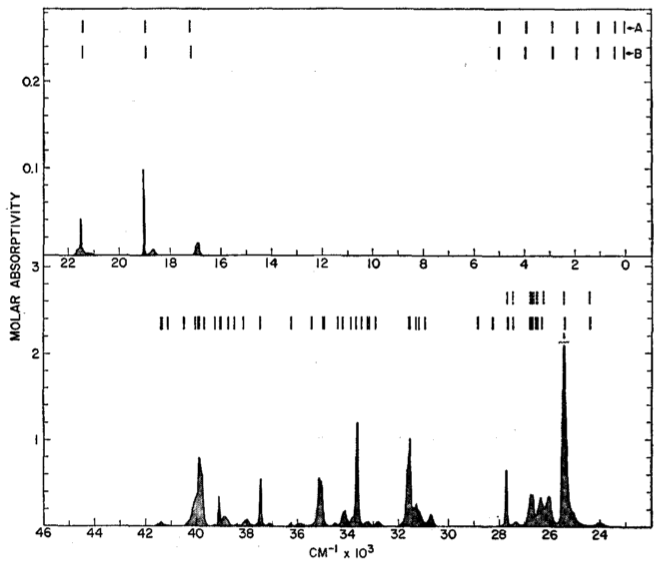
\includegraphics[width=\textwidth]{figures/eu_spec.png}
\end{center}
\caption[Aqueous Europium Spectrum from Literature]{The expected absorption spectrum of aqueous europium, taken directly from Carnall 1968\cite{Carnall:1968ch}. The weaker, forbidden transitions are mostly seen in the visible, there they have an order of magnitude lower molar extinction. The B line above the spectrum represents the theoretical electronic transitions calculated using \emph{ab initio} methods.}
\label{fig:eu_spec_theory}
\end{figure}

It is possible, using extensions to Judd-Ofelt calculations, to derive the
energy levels of the \textsl{4f} energy shell and the transitions from the
ground state of europium in different mediums
\cite{Carnall:1968ch,Carnall:1989fc,Richardson:1989vf,vanPieterson:2002hd}.

\begin{align}
  H = H_{\text{free ion}} + H_{CF} \label{eq:lan_ham}
\end{align}

%\begin{align*}
%H =\ & H_0 + \sum_{k=2,4,6} F^kf_k \\
 %& + \zeta(4f)A_{so} + \alpha L(L+1) + \beta G(G_2) + \gamma G(R_7)\\
 %& + \sum_{i=2,3,4,6,7,8}t_iT^i + \sum_{h=0,2,4}m_hM^h + \sum_{f=2,4,6}p_fP^f
%\end{align*}

This equation represents the free ion Hamiltonian of a lanthanide ion.
$H_{\text{free ion}}$ is the non-interacting electrons contribution (known as
the barycenter) \cite{Peijzel:2005jh}. Accurate quantum mechanical models of
the free ion term are available in the literature and can be easily solved
numerically on a computer \cite{Carnall:1989fc,Morrison:1988tw}.

One can then add perturbation terms to alter the Hamiltonian for use in
different solutions. For example, if the lanthanide is in a solid crystal
lattice, it is common to add

\begin{align*}
  H_{CF} = \sum_{k,q} B_q^k C_q^{(k)}
\end{align*}

which represents the radial $B$ and many-electron spherical tensor $C$ crystal
field interaction with the electron wave functions \cite{Peijzel:2005jh}.  Some
forbidden excited states of europium can also be understood through the
Wybourne-Downer mechanism, which accounts for spin-orbit interaction among
excited states and explicitly allows for $\Delta S = 1$ transitions to occur
\cite{Wybourne:1968ez,Downer:1988kz}.  Finally, Judd-Ofelt theory can be used
to estimate the transition intensities and branching ratios of absorption and
emission spectra, and therefore the natural radiative lifetimes
\cite{Werts:2002fs}.



\subsection{Measuring Radiative lifetimes of Europium Complexes using Fluorescence Emission}\label{subsec:rad_life}

The radiative lifetime of an electronic transition of an absorber can be
determined by its emission profile \cite{Werts:2002fs}. This is done through
the following formula.

\begin{align}
  \frac{1}{\tau_R} = \sum_JA_{J'J}\label{eq:nat_life_emiss}
\end{align}

In this formula, $A$ is the spontaneous emission probability of a particular
$J' \leftrightarrow J$ transition\marginpar{$A$ is also known as the Einstein
$A$ coefficient} (which is related to the area under the curve for that
emission peak), and $\tau_R$ is the ``natural'' radiative lifetime, which
is the lifetime of an electron in an excited state without interference
from systematic effects such as thermal quenching. Additionally, the
\emph{branching ratio} $\beta$ can be defined as the probability for an
excited electron to decay via a certain pathway $J_p$.

\begin{align}
  \beta_{J'J_P} = \dfrac{A_{J'J_p}}{\tau_R} = A_{J'J_p}\sum_J A_{J'J} \label{eq:branch_ratio}
\end{align}

For some absorbers, it can be difficult to measure all transitions
simultaneously, as some may be forbidden and hence extremely weak in comparison
to the allowed transitions. However, europium has a unique property that allows
its radiative lifetime to be determined from a single peak: europium contains a
single allowed magnetic dipole moment transition $^5D_0 \leftrightarrow ^7F_1$.
Magnetic dipole transitions are not affected by the solvent or complex that an
absorber is in, and hence this transition is constant \cite{Werts:2002fs}.
Using this peak, it is possible to measure the radiative lifetime using the
following equation

\begin{align}
  \dfrac{1}{\tau_R} = A_{MD,0}n^3\left(\frac{I}{I_{MD}}\right) \label{eq:nat_life_eu}
\end{align}

where $n$ is the refractive index of the solution, and the fraction
$\frac{I}{I_{MD}}$ is the ratio of the total area under the emission curve to
the area under just the $^5D_0 \leftrightarrow ^7F_1$ transition.

It is also possible, in cases where the absorption spectrum of a particular
luminescence transition is known, to calculate the radiative lifetime of the
transition \cite{Lewis:1945tp},

\begin{align}
  \frac{1}{\tau_R} = 2303 \dfrac{8\pi c n ^2 \nu^2}{N_A}\dfrac{g_l}{g_u}\int\epsilon(\nu)\,d\nu \label{eq:nat_life_abs}
\end{align}

where $\nu$ is the frequency of the transition, $\tfrac{g_l}{g_u}$ is the
fraction of electrons in the excited and ground state, and $\epsilon$ is the
molar extinction coefficient (in \iM\icm) of the transition.

\section*{Chapter Review}

Europium is a metal with a complicated electronic configuration that is not
fully understood at the time of writing. Theoretical investigations can
provide some indications to how europium ions will react to photons, but this
understanding is incomplete because of the strong response from ``forbidden''
transitions. Experimental tests must also be performed to attempt to create
an accurate model for europium's electronic transitions. Once the branching
ratios can be well predicted, their deviations from expected results can
be used to determine other particulates in a solution. This possibility is
discussed in chapter~\ref{ch:eu_exp}.
